\documentclass[conference]{IEEEtran}

\usepackage{cite}
\usepackage{amsmath,amssymb}
\usepackage{graphicx}
\usepackage{booktabs}
\usepackage{url}
\usepackage{tikz}
\usetikzlibrary{arrows.meta,positioning}

% A framed box that stands in for a photo until it is taken.
% Replace \placeholder{...} with \includegraphics[width=\columnwidth]{figures/<file>}.
\newcommand{\placeholder}[1]{%
  \fbox{\parbox[c][3.6cm][c]{0.92\columnwidth}{\centering\small\textbf{PHOTO PLACEHOLDER}\\[3pt]#1}}}

\newcommand{\vect}[1]{\boldsymbol{#1}}

\begin{document}

\title{Particle Filter Localization of a Mobile Robot\\with ArUco Markers and Wheel Odometry}

% TODO: fill in the team members' names and NetIDs.
\author{\IEEEauthorblockN{NAME 1 (NetID), NAME 2 (NetID), NAME 3 (NetID)}
\IEEEauthorblockA{Team 20, ROB-GY 6003 Foundations of Robotics\\
New York University Tandon School of Engineering\\
Brooklyn, NY, USA}}

\maketitle

% =====================================================================
\begin{abstract}
A mobile robot that knows its pose in a room can plan paths and return to places, but wheel odometry alone drifts without bound. We implemented a particle filter that estimates the planar pose of the LeKiwi omnidirectional robot in a map of ArUco markers. Odometry moves 2000 particles through a noisy motion model, and each marker the calibrated camera detects reweights them through a range, bearing and facing likelihood with an outlier cap, followed by low-variance resampling. We tested the filter in a simulated room with ground truth and on the real robot in a classroom with five mapped markers. The calibrated camera had a reprojection error of 0.41 px, and its marker distances were within 3.8\,\% of tape measurements from 0.5 to 3\,m. In simulation, starting with no knowledge of the pose, the position error fell below 20\,cm within 9.2\,s and averaged 8.9\,cm over a 115\,s run, while the odometry heading error grew to 5.8\,$^\circ$. On the real robot, the estimate was within 5.7 to 14.6\,cm (mean 9.1\,cm) of four tape-measured floor positions.
\end{abstract}

% =====================================================================
\section{Introduction}

Localization is the problem of finding a robot's pose with respect to a given map~\cite{clark6b}. Wheel odometry gives a smooth, fast estimate of how the robot moves, but every error in the measured wheel speeds is integrated and never corrected, so the pose drifts further the longer the robot drives. External landmarks with known positions do not drift, but they are only visible some of the time and each sighting is noisy. A Kalman filter fuses the two well when the belief is a single Gaussian~\cite{clark6b}. It cannot represent a robot that could be in several places, which is the situation at start-up when nothing is known, or when one landmark seen once is consistent with a whole circle of poses. A particle filter represents the belief with a set of weighted samples instead, so it can hold several hypotheses until later measurements rule them out~\cite{gordon1993,dellaert1999,thrun2005,clark7b}. Monte Carlo localization, the application of the particle filter to this problem, is the standard approach for mobile robots with landmark or range sensors~\cite{dellaert1999,thrun2005}.

This work localizes the LeKiwi, a low-cost three-wheeled omnidirectional robot built from serial-bus servos~\cite{lerobot}. Its landmarks are ArUco fiducial markers~\cite{garrido2014} printed and fixed to the walls of a classroom, whose positions were mapped beforehand. A front camera detects the markers, and the measured wheel speeds give odometry. The software runs as Robot Operating System~2 (ROS~2) nodes~\cite{macenski2022} that drive either a MuJoCo simulation~\cite{todorov2012} or the real robot~\cite{for26}.

The Method section (Section~\ref{sec:method}) gives the mathematical details of the camera calibration, of the marker detection and its conversion into a planar measurement, and of the particle filter: its state, motion model, measurement model and resampling, along with the design decisions behind them. The Experiment Design section (Section~\ref{sec:experiment}) describes the simulated and real setups and how the reference positions were measured. The Experimental Results section (Section~\ref{sec:results}) reports the calibration, the marker distance accuracy, the localization error over time, the consistency of detected markers with the map and the accuracy of the real robot at tape-measured spots, and discusses the problems we met. Section~\ref{sec:conclusion} summarizes the performance of the system.

% =====================================================================
\section{Method}
\label{sec:method}

\subsection{System overview}
Fig.~\ref{fig:block} shows the localization system. The wheel encoders give the base velocity, which an odometry node integrates into a dead-reckoned pose. The change in that pose between two messages is the control input $\vect{u}_t$ of the filter. The camera images go to an ArUco detector, which returns the pose of each visible marker relative to the camera. These detections are converted into planar measurements $\vect{z}_t$ in the robot's base frame. A map node supplies the marker positions in the map frame. The particle filter combines the three and publishes the estimated pose $\hat{\vect{X}}_t$ of the base in the map, with the spread of the particles as its covariance. All frames are right-handed with $z$ up; the base frame has $x$ forward and $y$ to the left.

\begin{figure}[t]
\centering
\resizebox{\columnwidth}{!}{%
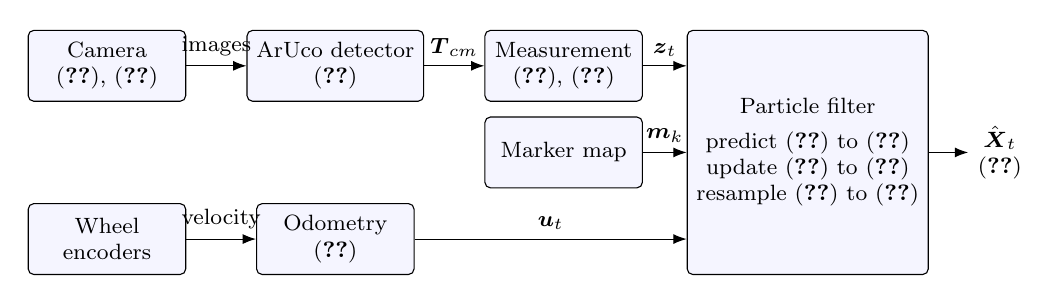
\begin{tikzpicture}[>=Latex, font=\footnotesize,
  box/.style={draw, rounded corners=2pt, align=center, minimum height=0.9cm, minimum width=2.0cm, fill=blue!4}]
  \node[box] (cam)  at (0, 1.1)  {Camera\\ \eqref{eq:pinhole}, \eqref{eq:distortion}};
  \node[box] (det)  at (2.9, 1.1) {ArUco detector\\ \eqref{eq:pnp}};
  \node[box] (meas) at (5.8, 1.1) {Measurement\\ \eqref{eq:base}, \eqref{eq:measurement}};
  \node[box] (whl)  at (0, -1.1) {Wheel\\ encoders};
  \node[box] (odo)  at (2.9, -1.1) {Odometry\\ \eqref{eq:control}};
  \node[box] (map)  at (5.8, 0) {Marker map};
  \node[box, minimum height=3.1cm, minimum width=2.3cm] (pf) at (8.9, 0)
       {Particle filter\\[3pt] predict \eqref{eq:noise} to \eqref{eq:propagate}\\ update \eqref{eq:expected} to \eqref{eq:weights}\\ resample \eqref{eq:neff} to \eqref{eq:jitter}};
  \node[right=0.5cm of pf, align=center] (out) {$\hat{\vect{X}}_t$\\ \eqref{eq:estimate}};
  \draw[->] (cam) -- node[above]{images} (det);
  \draw[->] (det) -- node[above]{$\vect{T}_{cm}$} (meas);
  \draw[->] (meas.east) -- node[above]{$\vect{z}_t$} (meas.east -| pf.west);
  \draw[->] (whl) -- node[above]{velocity} (odo);
  \draw[->] (odo.east) -- node[above]{$\vect{u}_t$} (odo.east -| pf.west);
  \draw[->] (map) -- node[above]{$\vect{m}_k$} (map -| pf.west);
  \draw[->] (pf) -- (out);
\end{tikzpicture}}
\caption{Block diagram of the localization system. Numbers in parentheses are the equations of Section~\ref{sec:method}.}
\label{fig:block}
\end{figure}

\subsection{Camera calibration}
A point $(X, Y, Z)$ in the camera frame ($x$ right in the image, $y$ down, $z$ along the optical axis) projects to the pixel $(u, v)$ of the pinhole model
\begin{equation}
\lambda \begin{bmatrix} u \\ v \\ 1 \end{bmatrix} =
\begin{bmatrix} f_x & 0 & c_x \\ 0 & f_y & c_y \\ 0 & 0 & 1 \end{bmatrix}
\begin{bmatrix} X \\ Y \\ Z \end{bmatrix},
\label{eq:pinhole}
\end{equation}
where $\lambda = Z$ is the depth, $f_x$ and $f_y$ are the focal lengths in pixels and $(c_x, c_y)$ is the principal point. The matrix is the camera matrix $\vect{K}$. The lens bends rays before they reach the sensor. With normalized coordinates $x_n = X/Z$, $y_n = Y/Z$ and $r^2 = x_n^2 + y_n^2$, the radial coefficients $k_1, k_2, k_3$ and the tangential coefficients $p_1, p_2$ give the distorted coordinates
\begin{equation}
\begin{aligned}
x_d &= x_n (1 + k_1 r^2 + k_2 r^4 + k_3 r^6) + 2 p_1 x_n y_n + p_2 (r^2 + 2 x_n^2),\\
y_d &= y_n (1 + k_1 r^2 + k_2 r^4 + k_3 r^6) + p_1 (r^2 + 2 y_n^2) + 2 p_2 x_n y_n.
\end{aligned}
\label{eq:distortion}
\end{equation}
The intrinsics $\vect{K}$ and $\vect{d} = [k_1, k_2, p_1, p_2, k_3]$ were estimated with Zhang's method~\cite{zhang2000} as implemented in OpenCV~\cite{bradski2000}: the inner corners of a planar checkerboard are detected in many images, and the intrinsics and the board pose in every image are adjusted together until the projected corners match the detected ones. The fit is measured by the root mean square reprojection error over all $M$ detected corners $\vect{q}_j$ and their projections $\hat{\vect{q}}_j$,
\begin{equation}
\epsilon = \sqrt{\frac{1}{M} \sum_{j=1}^{M} \left\| \vect{q}_j - \hat{\vect{q}}_j \right\|^2 }.
\label{eq:rms}
\end{equation}

\subsection{ArUco marker setup}
The markers come from the dictionary DICT\_4X4\_50: a $4 \times 4$ pattern of cells inside a black border, which encodes an id from 0 to 49~\cite{garrido2014}. The detector returns the id and the four corners of each marker in the image. In the marker's own frame ($x$ right, $y$ up, $z$ out of the printed side), the corners of a marker with edge length $s$ are
\begin{equation}
\vect{c}_{1,2,3,4} = \left(-\tfrac{s}{2}, \tfrac{s}{2}, 0\right), \left(\tfrac{s}{2}, \tfrac{s}{2}, 0\right), \left(\tfrac{s}{2}, -\tfrac{s}{2}, 0\right), \left(-\tfrac{s}{2}, -\tfrac{s}{2}, 0\right).
\label{eq:corners}
\end{equation}
The marker pose in the camera frame, a rotation $\vect{R}_{cm}$ and translation $\vect{t}_{cm}$, solves the perspective-$n$-point problem
\begin{equation}
(\vect{R}_{cm}, \vect{t}_{cm}) = \arg\min_{\vect{R}, \vect{t}} \sum_{k=1}^{4} \left\| \vect{q}_k - \pi\!\left(\vect{K}, \vect{d}, \vect{R}\vect{c}_k + \vect{t}\right) \right\|^2,
\label{eq:pnp}
\end{equation}
where $\vect{q}_k$ is the detected pixel of corner $k$ and $\pi$ is the projection of \eqref{eq:pinhole} and \eqref{eq:distortion}. We solve it with the IPPE method for squares~\cite{collins2014} and write the result as the homogeneous transform $\vect{T}_{cm}$. The camera's mounting pose on the robot, $\vect{T}_{bc}$, was measured (Section~\ref{sec:experiment}), so the marker in the base frame is
\begin{equation}
\vect{T}_{bm} = \vect{T}_{bc}\, \vect{T}_{cm}.
\label{eq:base}
\end{equation}

The filter state is planar, so each detection is reduced to three numbers in the floor plane: the range $\rho$ from the base centre to the marker, its bearing $\beta$ counter-clockwise from straight ahead, and its facing $\varphi$, the direction of the marker's $z$ axis. With $(m_x, m_y)$ the position and $(n_x, n_y)$ the planar part of the $z$ axis of $\vect{T}_{bm}$,
\begin{equation}
\vect{z} = \begin{bmatrix} \rho \\ \beta \\ \varphi \end{bmatrix} =
\begin{bmatrix} \sqrt{m_x^2 + m_y^2} \\ \operatorname{atan2}(m_y, m_x) \\ \operatorname{atan2}(n_y, n_x) \end{bmatrix}.
\label{eq:measurement}
\end{equation}
Range and bearing alone leave the robot anywhere on a circle around the marker. The facing, compared with the marker's mapped direction, fixes the robot's heading and with it the position on that circle, so one marker is enough for a full pose.

The map gives, for every marker $k$, its position and facing in the map frame, $\vect{m}_k = [x_k, y_k, \varphi_k]^T$. The classroom map was built by the course staff from phone videos with bundle adjustment~\cite{for26}; its origin is on the floor below marker~2, with $x$ pointing out of that marker's wall into the room.

\subsection{Particle filter}
\subsubsection{State, inputs and outputs}
Following the notation of~\cite{clark7b}, particle $i$ at time $t$ is a state and a weight,
\begin{equation}
\vect{p}_t^i = \begin{bmatrix} \vect{X}_t^i \\ w_t^i \end{bmatrix}, \qquad
\vect{X}_t^i = \begin{bmatrix} x_t^i \\ y_t^i \\ \theta_t^i \end{bmatrix},
\label{eq:particle}
\end{equation}
where $(x_t^i, y_t^i)$ is the position of the base centre in the map frame and $\theta_t^i$ its heading. The belief is the set $P_t = [\vect{p}_t^1, \dots, \vect{p}_t^N]$ of $N$ particles, with weights summing to one. Each cycle of the filter takes $P_{t-1}$, the odometry step $\vect{u}_t$ and the measurements $\vect{z}_t$, and returns $P_t$ and the pose estimate $\hat{\vect{X}}_t$. We write $\psi(\cdot)$ for wrapping an angle into $[-\pi, \pi)$.

\subsubsection{Initialization}
Nothing is known about the start pose, so the particles are drawn uniformly over the area $\mathcal{A}$ around the mapped markers (their bounding box grown by 0.5\,m) with uniform headings and equal weights~\cite{clark7b}:
\begin{equation}
(x_0^i, y_0^i) \sim \mathcal{U}(\mathcal{A}), \quad \theta_0^i \sim \mathcal{U}[-\pi, \pi), \quad w_0^i = \tfrac{1}{N}.
\label{eq:init}
\end{equation}
When a pose is known, the particles are drawn from a normal distribution around it instead.

\subsubsection{Motion model}
The odometry pose at time $t$ is the planar homogeneous transform $\vect{T}_t$ in the odometry frame. The step since the previous message, expressed in the robot's frame at the start of the step, is
\begin{equation}
\vect{u}_t = \begin{bmatrix} \Delta x_t \\ \Delta y_t \\ \Delta\theta_t \end{bmatrix} \leftarrow \vect{T}_{t-1}^{-1}\, \vect{T}_t,
\label{eq:control}
\end{equation}
where $\Delta x_t$ is forward, $\Delta y_t$ to the left and $\Delta\theta_t$ the turn. The odometry error grows with the size of the step, so the standard deviations of the translational and rotational noise are
\begin{equation}
\sigma_{s} = \alpha_1 \sqrt{\Delta x_t^2 + \Delta y_t^2} + \sigma_{1}, \qquad
\sigma_{r} = \alpha_2 \left|\Delta\theta_t\right| + \sigma_{2},
\label{eq:noise}
\end{equation}
with proportional gains $\alpha_1, \alpha_2$ and floors $\sigma_1, \sigma_2$. Every particle draws its own noisy step,
\begin{equation}
\delta x^i \sim \mathcal{N}(\Delta x_t, \sigma_s^2), \quad
\delta y^i \sim \mathcal{N}(\Delta y_t, \sigma_s^2), \quad
\delta\theta^i \sim \mathcal{N}(\Delta\theta_t, \sigma_r^2),
\label{eq:sample}
\end{equation}
and applies it in its own frame:
\begin{equation}
\begin{aligned}
x_t^i &= x_{t-1}^i + \delta x^i \cos\theta_{t-1}^i - \delta y^i \sin\theta_{t-1}^i,\\
y_t^i &= y_{t-1}^i + \delta x^i \sin\theta_{t-1}^i + \delta y^i \cos\theta_{t-1}^i,\\
\theta_t^i &= \psi\!\left(\theta_{t-1}^i + \delta\theta^i\right).
\end{aligned}
\label{eq:propagate}
\end{equation}
The lecture's example samples a differential-drive robot by perturbing the two wheel distances and moving along the mid-step heading~\cite{clark7b}. The LeKiwi has omnidirectional wheels and can move sideways, so we perturb the planar step $\vect{u}_t$ directly and use the same noise level forward and sideways.

\subsubsection{Measurement model}
A particle at $(x, y, \theta)$ that sees marker $k$ expects to measure
\begin{equation}
\hat{\rho} = \sqrt{(x_k - x)^2 + (y_k - y)^2}, \quad
\hat{\beta} = \psi\!\left(\operatorname{atan2}(y_k - y, x_k - x) - \theta\right), \quad
\hat{\varphi} = \psi(\varphi_k - \theta).
\label{eq:expected}
\end{equation}
The errors are modelled as independent and normal. A marker further away covers fewer pixels, so its range and facing are less certain; the standard deviations of those two grow with the measured range. The normalized errors are
\begin{equation}
e_\rho = \frac{\rho - \hat{\rho}}{\kappa_\rho\, \rho}, \quad
e_\beta = \frac{\psi(\beta - \hat{\beta})}{\sigma_\beta}, \quad
e_\varphi = \frac{\psi(\varphi - \hat{\varphi})}{\kappa_\varphi\, \rho},
\label{eq:errors}
\end{equation}
where $\kappa_\rho$ is the range error as a fraction of the range, $\sigma_\beta$ the bearing standard deviation and $\kappa_\varphi$ the facing standard deviation per metre. The likelihood of a measurement is computed as a logarithm, so that the product over several markers becomes a sum and does not underflow. Each normalized error is capped at $\gamma$ standard deviations:
\begin{equation}
\ell^i = -\frac{1}{2} \sum_{k \in \mathcal{K}_t} \sum_{e \in \{e_\rho, e_\beta, e_\varphi\}} \min\!\left(|e|, \gamma\right)^2,
\label{eq:loglik}
\end{equation}
where $\mathcal{K}_t$ is the set of detected markers that are in the map and closer than $\rho_{\max}$. The cap makes the filter tolerate a bad detection, such as a misread id or a flipped orientation. Without it, one error of ten standard deviations would multiply the weight of every correct particle by $e^{-50}$, and the filter would jump to wherever the bad detection happens to fit. The new weights are
\begin{equation}
w_t^i = \frac{w_{t-1}^i\, \exp(\ell^i)}{\sum_{j=1}^{N} w_{t-1}^j\, \exp(\ell^j)}.
\label{eq:weights}
\end{equation}
The constant factor of the normal density is the same for all particles and cancels in \eqref{eq:weights}, as noted in~\cite{clark7b}.

\subsubsection{Resampling}
Resampling discards particles that no longer explain the measurements and copies likely ones. It also loses information about less likely hypotheses, so the filter resamples only after a measurement update~\cite{clark7b} and only when the weights have become uneven, measured by the effective number of particles~\cite{thrun2005}:
\begin{equation}
N_{\mathrm{eff}} = \frac{1}{\sum_{i=1}^{N} (w_t^i)^2} < \eta N.
\label{eq:neff}
\end{equation}
We use low-variance (systematic) resampling~\cite{kitagawa1996,thrun2005}. With the cumulative weights $C_i = \sum_{j=1}^{i} w_t^j$, one random number $r$ places $N$ equally spaced pointers $\mu_n$, and each picks the particle whose interval contains it:
\begin{equation}
r \sim \mathcal{U}\!\left[0, \tfrac{1}{N}\right), \quad \mu_n = r + \frac{n-1}{N}, \quad
i_n = \min \{ i : C_i \geq \mu_n \}.
\label{eq:lowvar}
\end{equation}
A particle with weight $w$ is copied either $\lfloor N w \rfloor$ or $\lceil N w \rceil$ times. The roulette-wheel scheme of~\cite{clark7b} draws $N$ independent random numbers and can drop a good particle or copy a poor one by chance; one random number removes that variance. Copies of one particle are identical, so after resampling every particle is moved by a small jitter,
\begin{equation}
x_t^i \mathrel{+}= \epsilon_x, \quad y_t^i \mathrel{+}= \epsilon_y, \quad \theta_t^i \mathrel{+}= \epsilon_\theta, \qquad
\epsilon_{x,y} \sim \mathcal{N}(0, \sigma_j^2), \ \epsilon_\theta \sim \mathcal{N}(0, \sigma_{j\theta}^2),
\label{eq:jitter}
\end{equation}
and a fraction $\zeta$ of the particles is replaced by particles drawn from \eqref{eq:init}. These random particles let the filter recover if every particle is wrong, for example after the robot is carried to a new place.

\subsubsection{Estimate and update schedule}
The estimate is the particle with the largest weight,
\begin{equation}
\hat{\vect{X}}_t = \vect{X}_t^{i^*}, \qquad i^* = \arg\max_i w_t^i.
\label{eq:estimate}
\end{equation}
When the particles form two clusters, the weighted mean lies between them, where no particle is; the best particle always lies in one of them. The camera delivers about 30 images per second, and detections of a marker taken while the robot stands still share the same error, so treating them as independent would make the filter overconfident~\cite{thrun2005}. The update \eqref{eq:expected} to \eqref{eq:jitter} therefore runs only when the robot has moved or enough time has passed since the last update:
\begin{equation}
\sqrt{\delta_x^2 + \delta_y^2} \geq d_{\min} \ \lor\ |\delta_\theta| \geq \theta_{\min} \ \lor\ \tau \geq \tau_{\max},
\label{eq:schedule}
\end{equation}
where $(\delta_x, \delta_y, \delta_\theta)$ is the odometry motion and $\tau$ the time since the last update. The prediction runs on every odometry message. Table~\ref{tab:params} lists the parameters.

\begin{table}[t]
\centering
\caption{Particle filter parameters}
\label{tab:params}
\begin{tabular}{@{}lll@{}}
\toprule
Symbol & Meaning & Value \\
\midrule
$N$ & number of particles & 2000 \\
$\alpha_1, \alpha_2$ & motion noise gains \eqref{eq:noise} & 0.1, 0.1 \\
$\sigma_1, \sigma_2$ & motion noise floors \eqref{eq:noise} & 2\,mm, 0.002\,rad \\
$\kappa_\rho$ & range error fraction \eqref{eq:errors} & 0.1 \\
$\sigma_\beta$ & bearing standard deviation \eqref{eq:errors} & 0.087\,rad (5\,$^\circ$) \\
$\kappa_\varphi$ & facing error per metre \eqref{eq:errors} & 0.1\,rad/m \\
$\gamma$ & outlier cap \eqref{eq:loglik} & 3 \\
$\rho_{\max}$ & largest range used & 5\,m \\
$\eta$ & resampling threshold \eqref{eq:neff} & 0.5 \\
$\sigma_j, \sigma_{j\theta}$ & jitter \eqref{eq:jitter} & 1\,cm, 0.01\,rad \\
$\zeta$ & random particle fraction & 0.01 \\
$d_{\min}, \theta_{\min}, \tau_{\max}$ & update schedule \eqref{eq:schedule} & 2\,cm, 0.03\,rad, 1\,s \\
\bottomrule
\end{tabular}
\end{table}

% =====================================================================
\section{Experiment Design}
\label{sec:experiment}

\subsection{Simulation}
The simulator renders the robot's front camera at $640 \times 480$ pixels as an ideal pinhole camera with a 70\,$^\circ$ vertical field of view, in a $6 \times 5$\,m room with ten markers on its walls at a height of 0.25\,m~\cite{for26}. It adds a 5\,\% error to the wheel odometry and publishes the true pose of the robot, which serves as ground truth. With the true position $(x^*, y^*)$ and heading $\theta^*$, the position and heading errors of an estimate are
\begin{equation}
e_p = \sqrt{(\hat{x} - x^*)^2 + (\hat{y} - y^*)^2}, \qquad
e_\theta = \left| \psi(\hat{\theta} - \theta^*) \right|.
\label{eq:poserror}
\end{equation}
The robot started at the map origin and drove a 1.5\,m square twice at 0.15\,m/s, a 115\,s run. The run was recorded twice. In the first, the particles started uniformly over the room \eqref{eq:init} (unknown start). In the second, they started around the true pose with standard deviations of 5\,cm and 0.055\,rad (known start). Because the odometry frame starts at the robot's start pose, which is the map origin, the odometry pose can be compared directly with the truth.

To measure marker consistency, every detected marker was placed in the map through the current estimate, $\hat{\vect{T}}_{mb} \vect{T}_{bm}$, and compared with its mapped position. The marker error is the planar distance
\begin{equation}
e_m = \sqrt{(\hat{m}_x - x_k)^2 + (\hat{m}_y - y_k)^2},
\label{eq:markererror}
\end{equation}
recorded against the range $\rho$ while the robot drove the same square after a turn on the spot to converge.

\subsection{Real robot and classroom}
Fig.~\ref{fig:map} shows the classroom map. Five markers with ids 1, 2, 4, 7 and 8 hang at a height of 0.24\,m; their black squares are 206.5\,mm wide. The same nodes ran on the robot's computer, with the robot driver in place of the simulator~\cite{for26,lerobot}. Fig.~\ref{fig:robot} shows the robot in the classroom.

\begin{figure}[t]
\centering
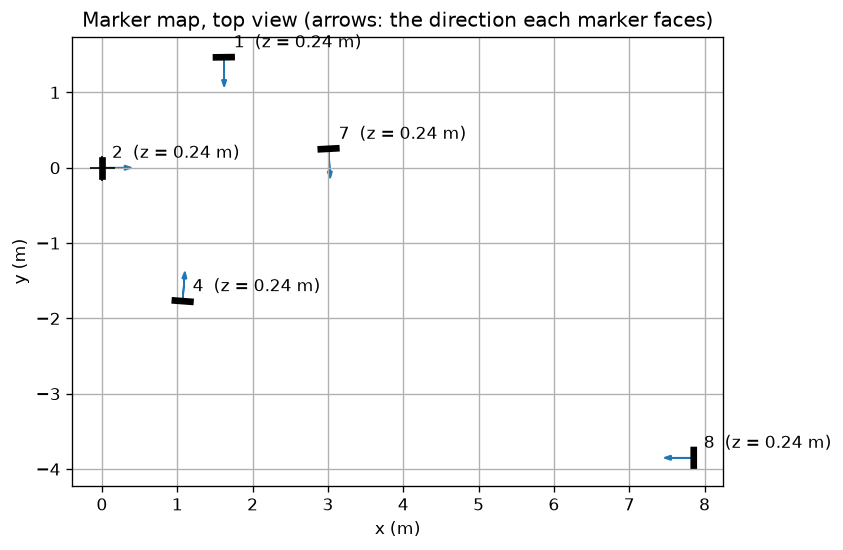
\includegraphics[width=\columnwidth]{figures/classroom_map.png}
\caption{Classroom marker map, top view~\cite{for26}. Arrows show the direction each marker faces. The origin is on the floor below marker~2.}
\label{fig:map}
\end{figure}

\begin{figure}[t]
\centering
\placeholder{Photo: the LeKiwi robot on the classroom floor, with wall markers visible behind it.}
\caption{The LeKiwi robot in the classroom.}
\label{fig:robot}
\end{figure}

\subsubsection{Camera calibration}
A checkerboard of $11 \times 8$ squares ($10 \times 7$ inner corners) was printed; the print came out at about 70\,\% scale, so its squares were about 17.5\,mm. The square size only sets the distance to the board in each image and does not change the intrinsics. Thirty-three images at $640 \times 480$ pixels were taken with the robot's camera, with the board placed in the corners and along the edges of the image, tilted by up to about 45\,$^\circ$, and at several distances.

\subsubsection{Camera mount}
The lens position relative to the base centre (the midpoint of the three wheels) was measured with a tape measure: 0.132\,m forward, on the centre line, and 0.043\,m above the base frame origin. The upward tilt, first estimated at 12\,$^\circ$, was refined to 9.6\,$^\circ$ using the distance experiment below.

\subsubsection{Marker distance}
A marker was placed upright, facing the camera, at tape-measured floor distances of 0.5 to 3.0\,m from the point below the lens; the room did not allow longer distances. At each distance, 2\,s of detections (about 70) were averaged. The detector reports the straight line from the lens to the marker centre, and the marker centre was higher than the lens, so the horizontal distance was compared, computed with the camera tilt.

\subsubsection{Real-robot accuracy}
Four spots were marked with tape crosses on the classroom floor (Fig.~\ref{fig:spots}). A tape measure was laid from the point on the floor below marker~2, perpendicular to its wall, as the $x$ axis; the $y$ coordinates were measured perpendicular to it. The robot was driven with its base centre over each cross, facing marker~2, and 10\,s of the pose estimate were averaged. Detected markers were also recorded while the robot drove through the room for about 75\,s, for the real-robot marker consistency.

\begin{figure}[t]
\centering
\placeholder{Photo: the tape crosses on the floor, the tape measure along the $x$ axis from below marker~2, and the robot on a cross.}
\caption{Floor spots for the real-robot accuracy test, measured from the point below marker~2.}
\label{fig:spots}
\end{figure}

% =====================================================================
\section{Experimental Results}
\label{sec:results}

\subsection{Camera calibration}
Table~\ref{tab:calib} gives the calibrated intrinsics, and Fig.~\ref{fig:calib} shows one of the 33 images with its detected corners. The reprojection error \eqref{eq:rms} was 0.41\,px (worst image 0.62\,px), below the 0.5\,px usually considered good. The focal lengths differ by 0.1\,\%, so the pixels are square. The principal point lies 24\,px right of and below the image centre, which means the lens is slightly off-centre over the sensor. The field of view is 86.9\,$^\circ$ by 70.8\,$^\circ$, as expected for a wide-angle camera.

\begin{table}[t]
\centering
\caption{Calibrated camera intrinsics}
\label{tab:calib}
\begin{tabular}{@{}ll@{}}
\toprule
Quantity & Value \\
\midrule
Image size & $640 \times 480$ px \\
$f_x, f_y$ & 337.9, 337.5 px \\
$c_x, c_y$ & 344.1, 264.1 px \\
$k_1, k_2, k_3$ & 0.0318, $-0.0693$, 0.0180 \\
$p_1, p_2$ & 0.0032, 0.0018 \\
RMS error $\epsilon$ & 0.41 px (worst image 0.62 px) \\
Field of view & 86.9\,$^\circ$ horizontal, 70.8\,$^\circ$ vertical \\
\bottomrule
\end{tabular}
\end{table}

\begin{figure}[t]
\centering
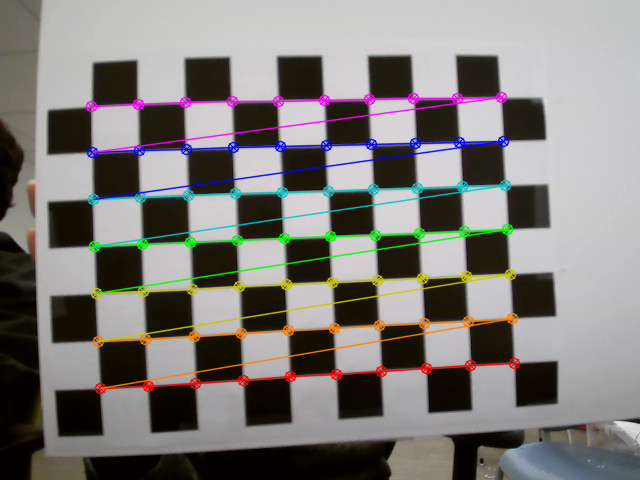
\includegraphics[width=0.85\columnwidth]{figures/calibration_corners.png}
\caption{A calibration image with the 70 detected inner corners of the checkerboard.}
\label{fig:calib}
\end{figure}

\subsection{Marker distance accuracy}
Fig.~\ref{fig:distance} compares the detected and tape-measured distances. The error grows with the distance, from $+11$\,mm at 0.5\,m to $+115$\,mm at 3\,m. A line fit gives $-11$\,mm plus 3.7\,\% of the distance, so the error is mostly proportional. A proportional error in a monocular estimate means a scale error: the distance follows from the apparent size of a marker of assumed size $s$ through the focal length, so a marker smaller than assumed or a focal length that is too large lengthens every distance by the same factor. The measured marker was $207 \times 210$\,mm, close to the assumed 206.5\,mm, which points to the focal length. The board was printed on paper and not glued down, and a curved board is a known cause of a biased focal length. The spread of the detections grew from 0.2\,mm at 0.5\,m to 29\,mm at 3\,m, as the marker shrank in the image. A reading at 1.5\,m was discarded because a second marker in view was averaged with the first.

The marker was detected at every distance tested, up to 3.0\,m, where its image was about 22\,px wide ($f_x s / \rho$); the room did not allow a test of the maximum range. The experiment also gave the camera tilt. The marker stayed at the same height, but with a tilt of 12\,$^\circ$ its computed height above the lens rose from 23 to 36\,cm with distance. A tilt of 9.6\,$^\circ$ makes the computed height constant at about 21\,cm, and that value was used afterwards.

\begin{figure*}[t]
\centering
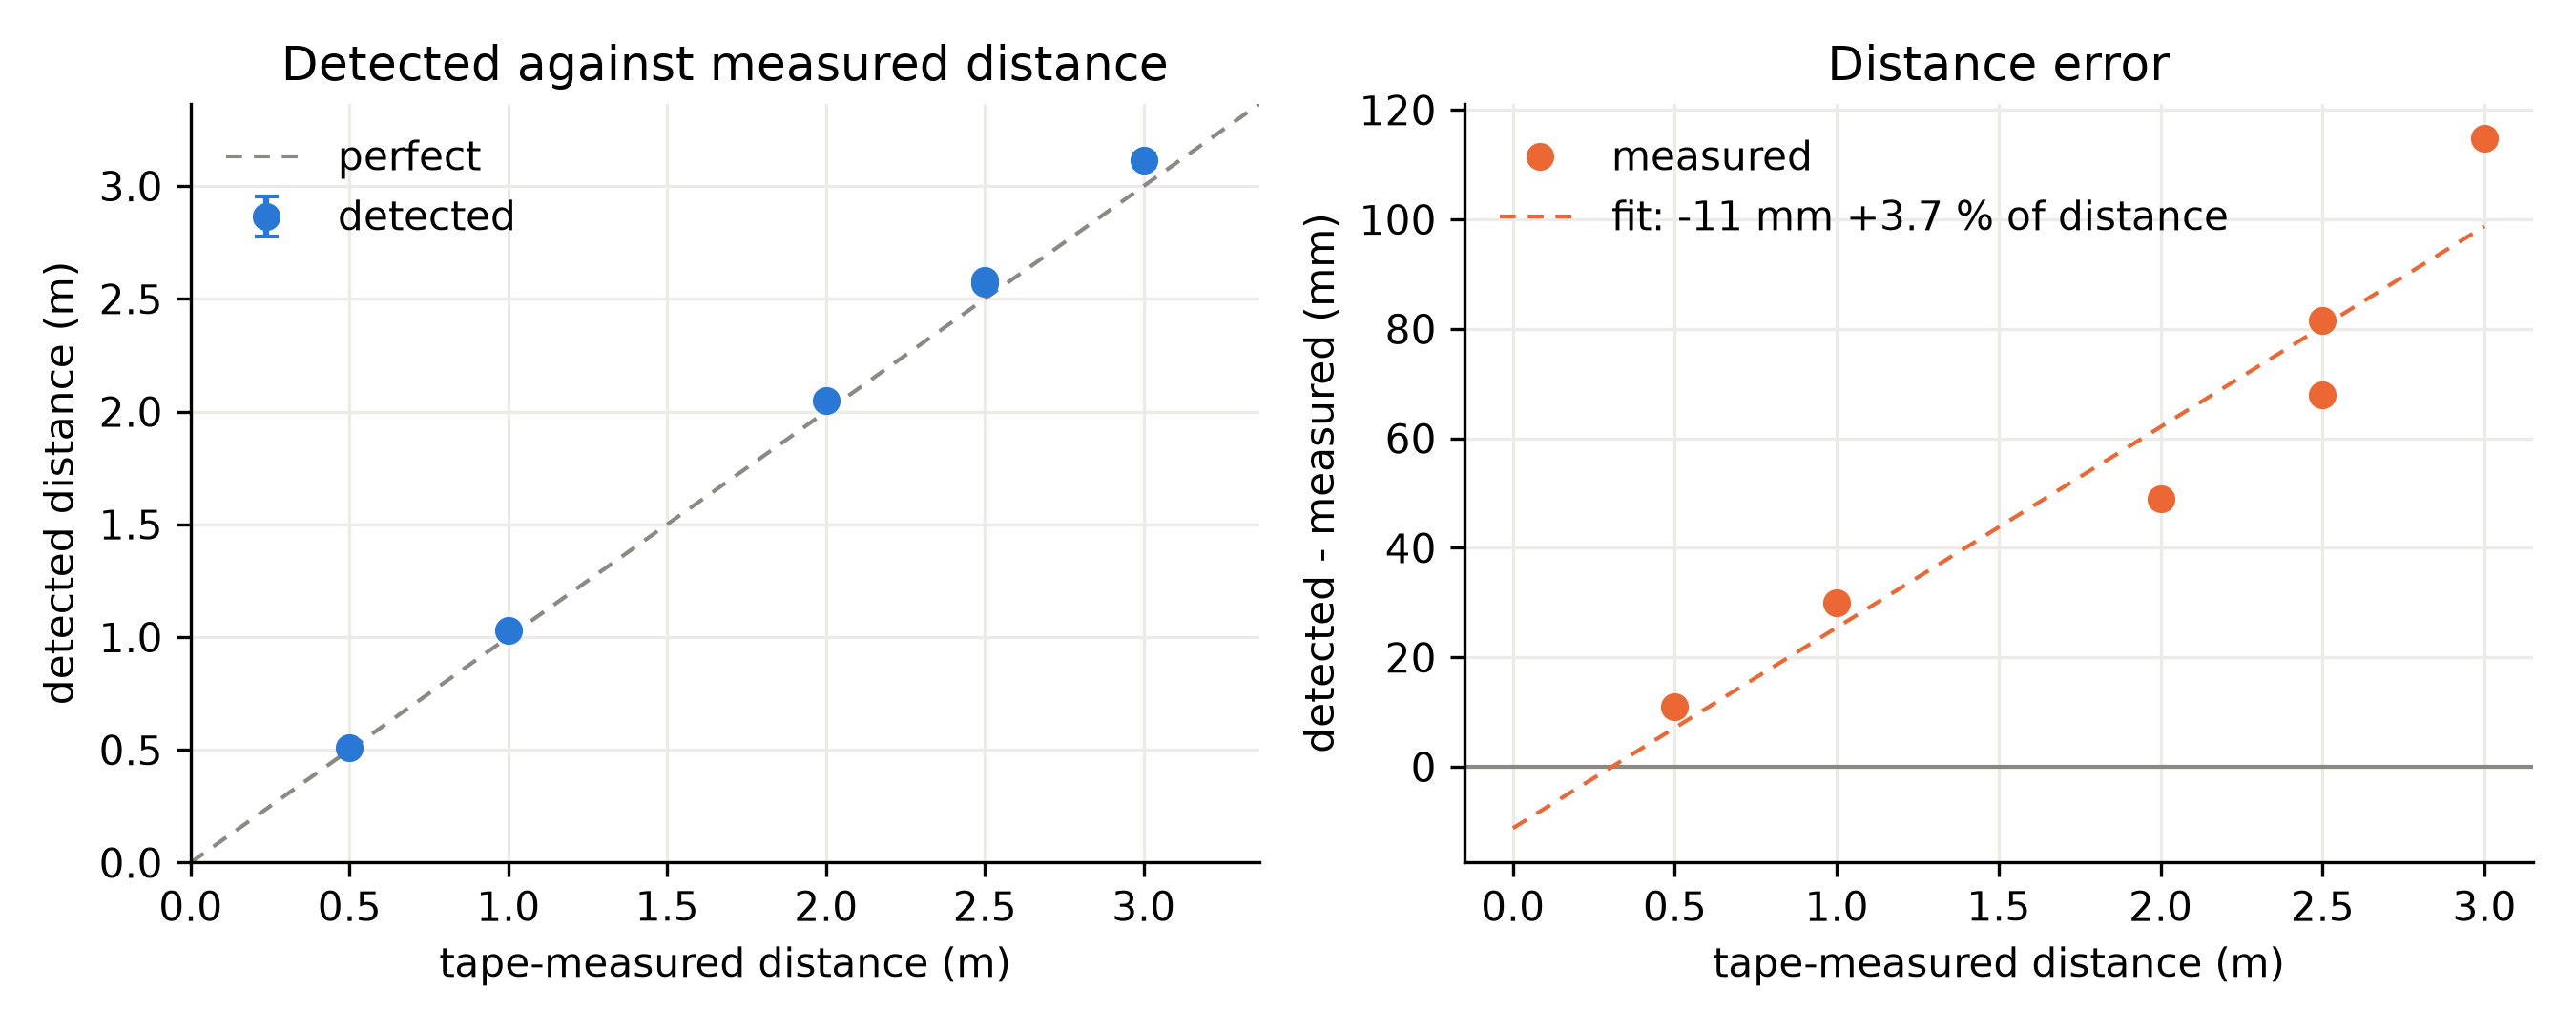
\includegraphics[width=0.8\textwidth]{figures/distance_accuracy.png}
\caption{Real camera: detected against tape-measured marker distance (left) and the distance error with a line fit (right). Error bars are the standard deviation of about 70 detections.}
\label{fig:distance}
\end{figure*}

\subsection{Localization accuracy in simulation}
Fig.~\ref{fig:l1} shows the position and heading errors \eqref{eq:poserror} over time, and Table~\ref{tab:l1} summarizes them. With an unknown start, the error began near 1\,m because the particles covered the whole room. It fell below 20\,cm within 9.2\,s and stayed there for the rest of the run. With a known start, the error was below 18.3\,cm throughout. After about 20\,s the two runs were indistinguishable, so once the filter converged, the initial belief no longer mattered. The heading error of both runs rose to about 5\,$^\circ$ at each corner of the square, where the robot turns in place, and fell again on the straight sides.

The odometry error grew steadily. Its heading error reached 5.8\,$^\circ$ and its position error 11.2\,cm at the end of the run, and odometry has no way to reduce either. For the first minute the odometry error was smaller than that of the filter, because odometry started exactly at the true pose while the filter's estimate jumped by a few centimetres between neighbouring particles.

\begin{figure}[t]
\centering
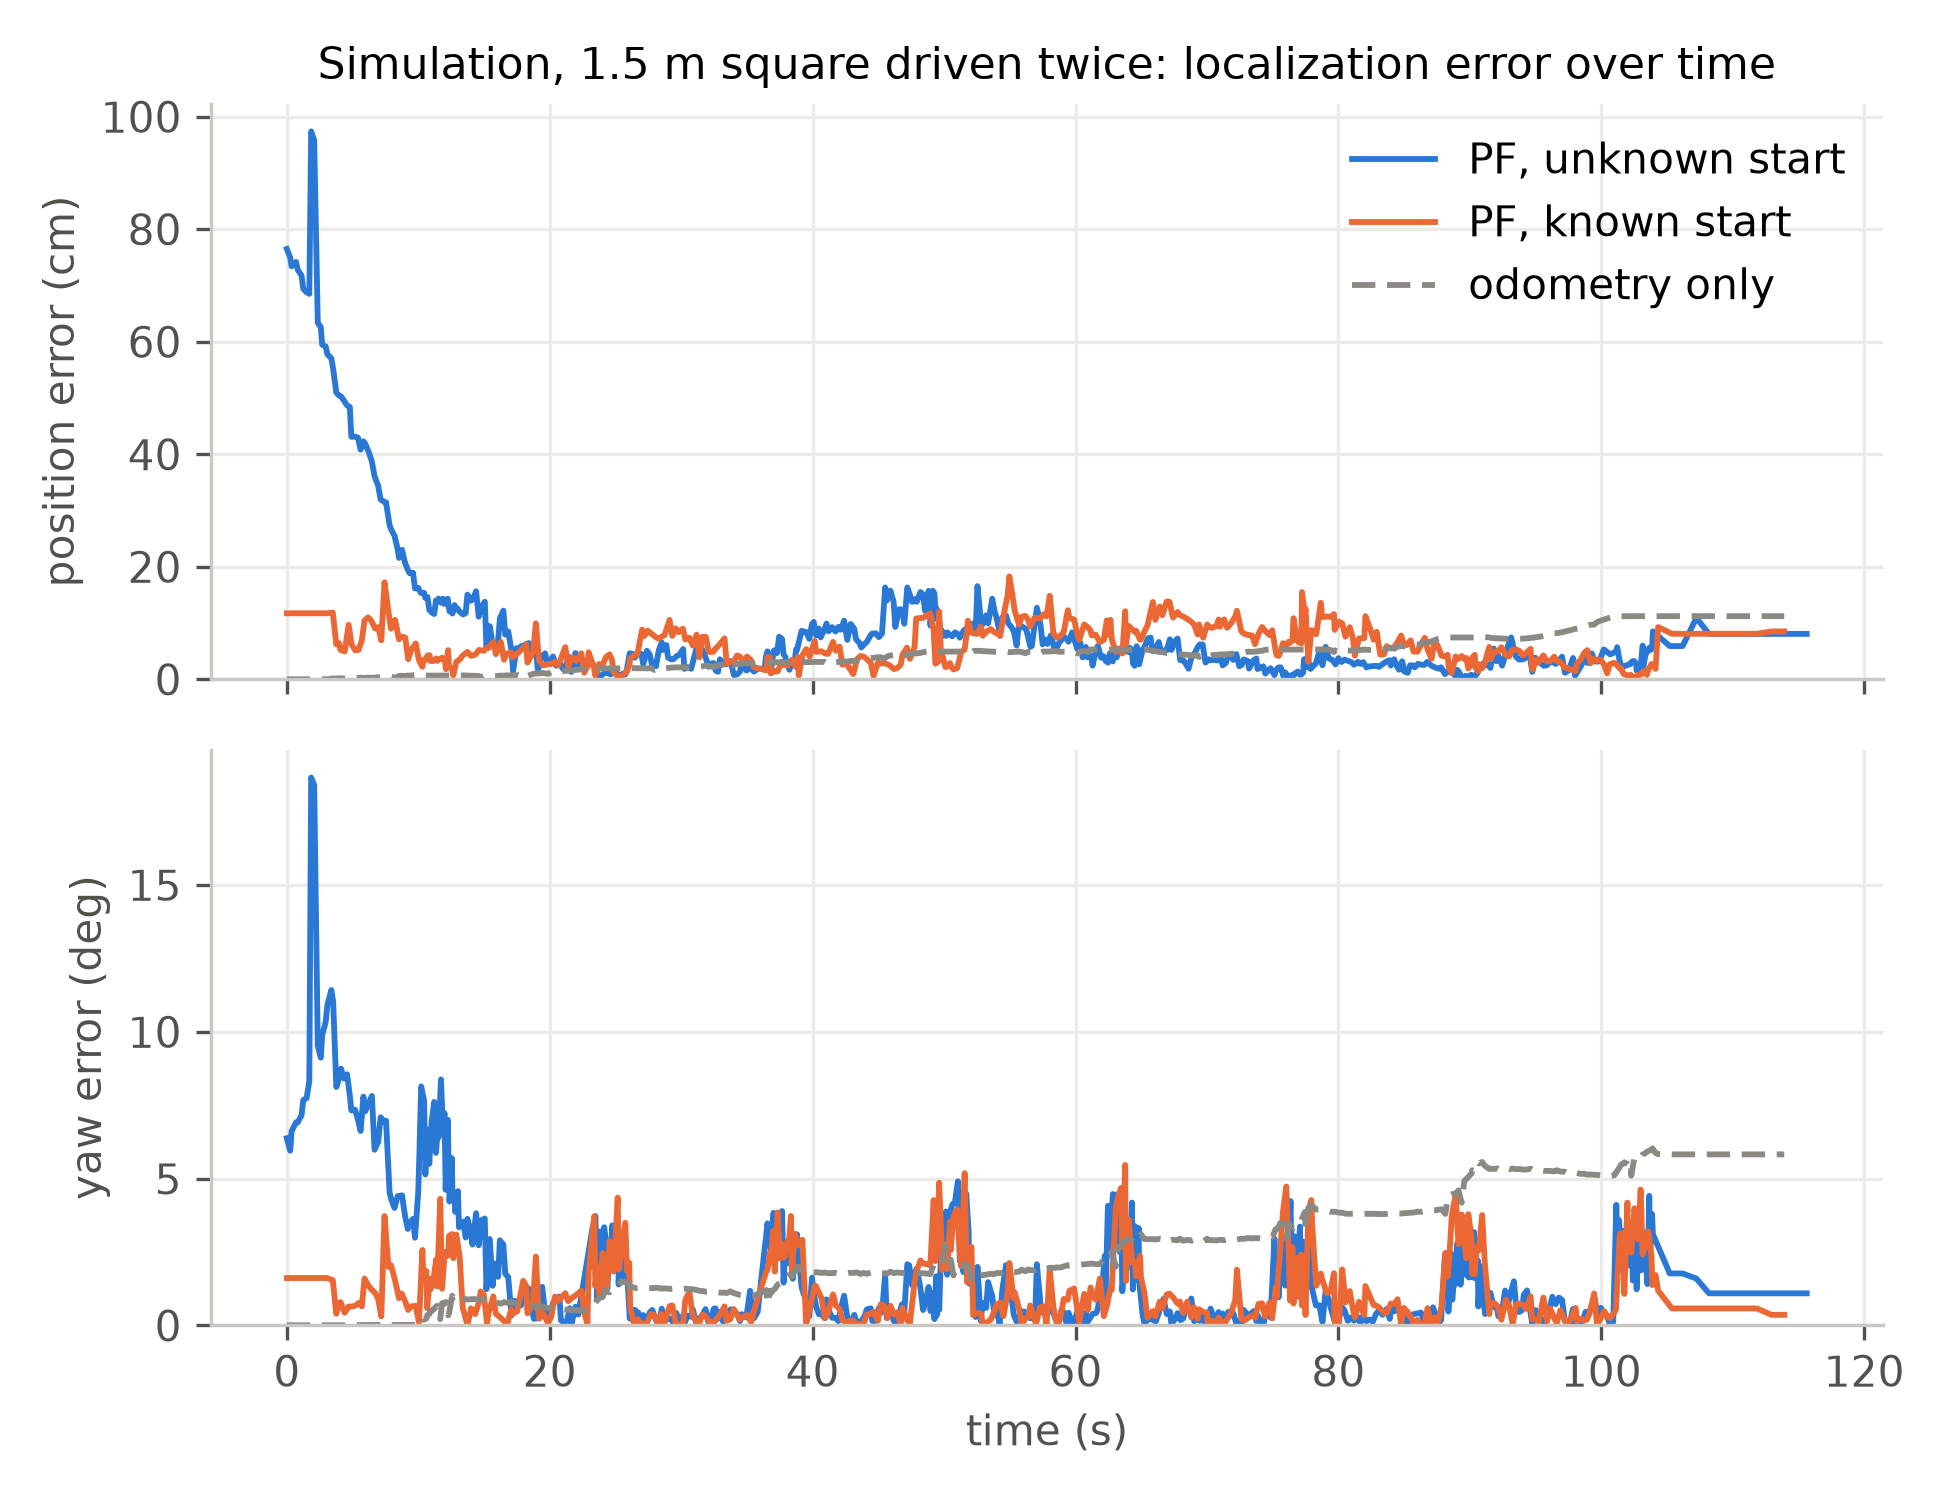
\includegraphics[width=\columnwidth]{figures/l1_error_over_time.png}
\caption{Simulation, 1.5\,m square driven twice: position error (top) and heading error (bottom) of the particle filter with unknown and known start, and of odometry alone.}
\label{fig:l1}
\end{figure}

\begin{table}[t]
\centering
\caption{Simulation errors over the 115\,s square run (mean / max / final)}
\label{tab:l1}
\setlength{\tabcolsep}{4pt}
\begin{tabular}{@{}lll@{}}
\toprule
 & Position (cm) & Heading ($^\circ$) \\
\midrule
PF, unknown start & 8.9 / 97.4 / 8.1 & 1.9 / 18.7 / 1.1 \\
PF, known start & 6.0 / 18.3 / 8.5 & 1.2 / 5.5 / 0.4 \\
Odometry & 4.5 / 11.2 / 11.2 & 2.5 / 6.0 / 5.8 \\
\bottomrule
\end{tabular}
\end{table}

\subsection{Marker consistency}
Fig.~\ref{fig:l2} plots the marker error \eqref{eq:markererror} against the distance to the marker. In simulation (1025 detections of all ten markers), the median error grew from 0.8\,cm at 0.5 to 1\,m to 2.8\,cm at 2.5 to 3\,m and 7.0\,cm at 4.5 to 5\,m. The growth matches the distance experiment: a far marker covers fewer pixels, so its range and facing are less certain, which is why the measurement model scales $\kappa_\rho \rho$ and $\kappa_\varphi \rho$ with the range. No marker was off at every distance; marker 19 had the largest median, 8.9\,cm, because it was only seen from 4.3 to 5\,m. A few detections were off by about 25\,cm, the kind of outlier that the cap $\gamma$ limits.

On the real robot (342 detections of markers 1, 2, 4 and 7, at 0.9 to 2\,m), the median error was 1.3\,cm up to 1.5\,m and 6.0\,cm from 1.5 to 2\,m. Markers 2 and 4 agreed with the map to a median of 1.4 and 1.2\,cm. Markers 1 and 7 had medians of 6.5 and 7.7\,cm. They were only seen from 1.6 to 1.8\,m, where the simulated median was 1.5\,cm, so the real errors at that distance were about four times larger. With 82 detections from one part of the room, the data cannot tell whether this comes from the map positions of these two markers, from the detection at that range, or from the pose estimate.

\begin{figure}[t]
\centering
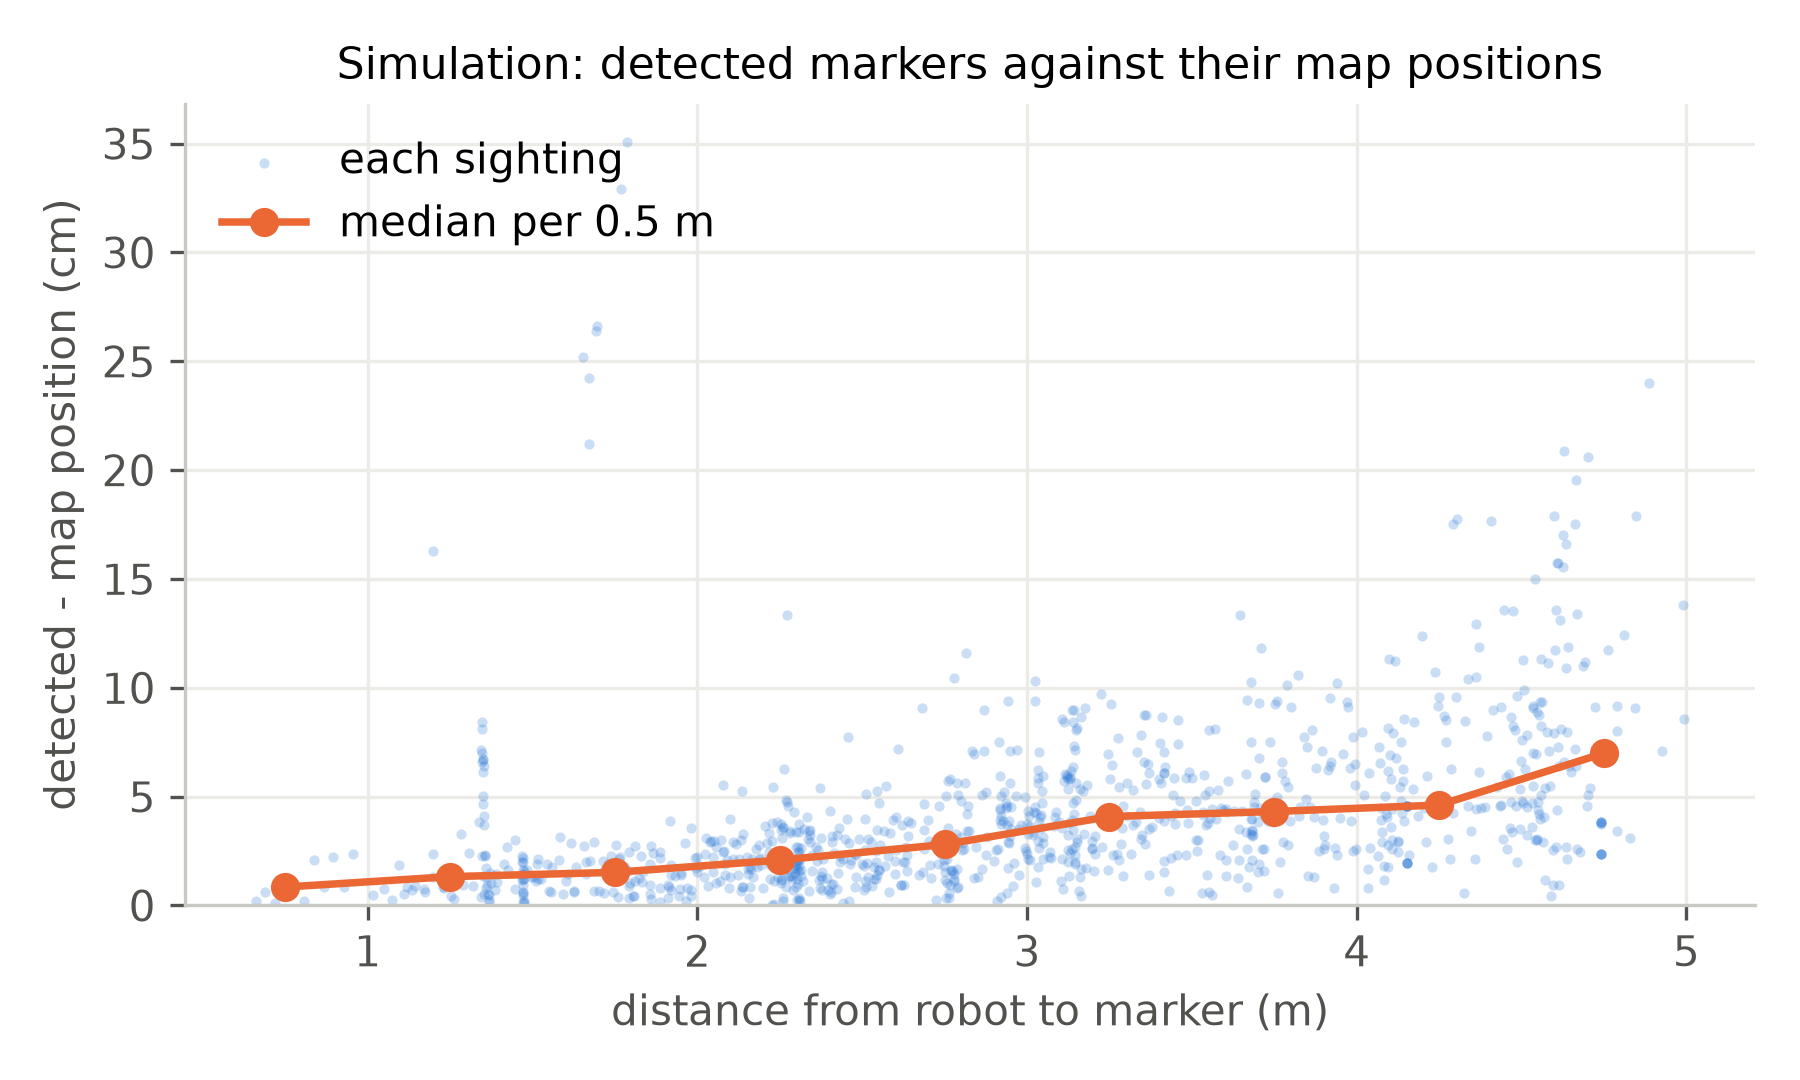
\includegraphics[width=\columnwidth]{figures/l2_sim.png}\\[2pt]
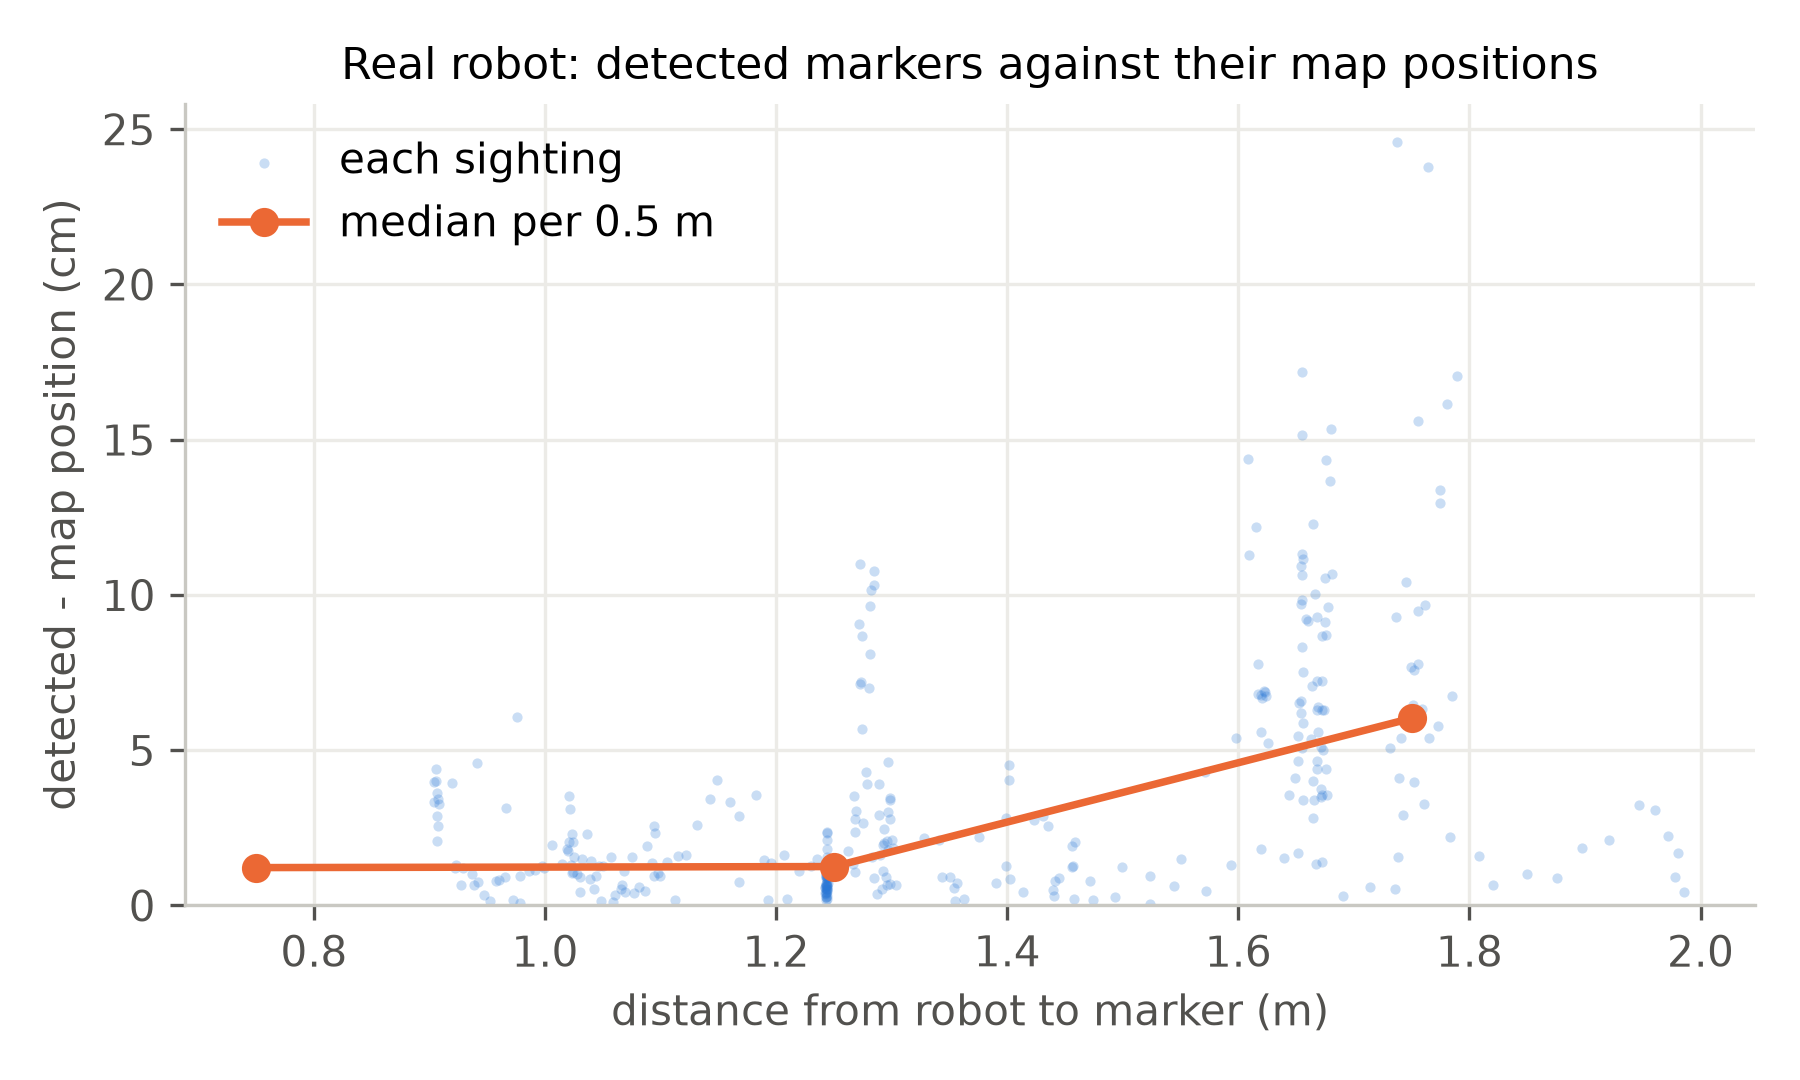
\includegraphics[width=\columnwidth]{figures/l2_real.png}
\caption{Distance of each detected marker from its mapped position, against the distance from the robot: simulation (top) and real robot (bottom). The orange line is the median in 0.5\,m bins.}
\label{fig:l2}
\end{figure}

\subsection{Real-robot accuracy}
Fig.~\ref{fig:spots_result} and Table~\ref{tab:l3} compare the estimates with the tape-measured spots. The errors were 5.7 to 14.6\,cm, with a mean of 9.1\,cm, similar to the simulated mean of 6.0 to 8.9\,cm. While the robot stood still, the estimate varied by 0.9 to 7.6\,cm. Spot~4, 2\,m from marker~2, had the largest error, mostly sideways ($-14$\,cm in $y$), consistent with the larger errors of more distant detections. The estimated headings (150 to 177\,$^\circ$, or $-160$\,$^\circ$) agree with the robot facing marker~2 in the $-x$ direction, which corresponds to 180\,$^\circ$.

\begin{figure}[t]
\centering
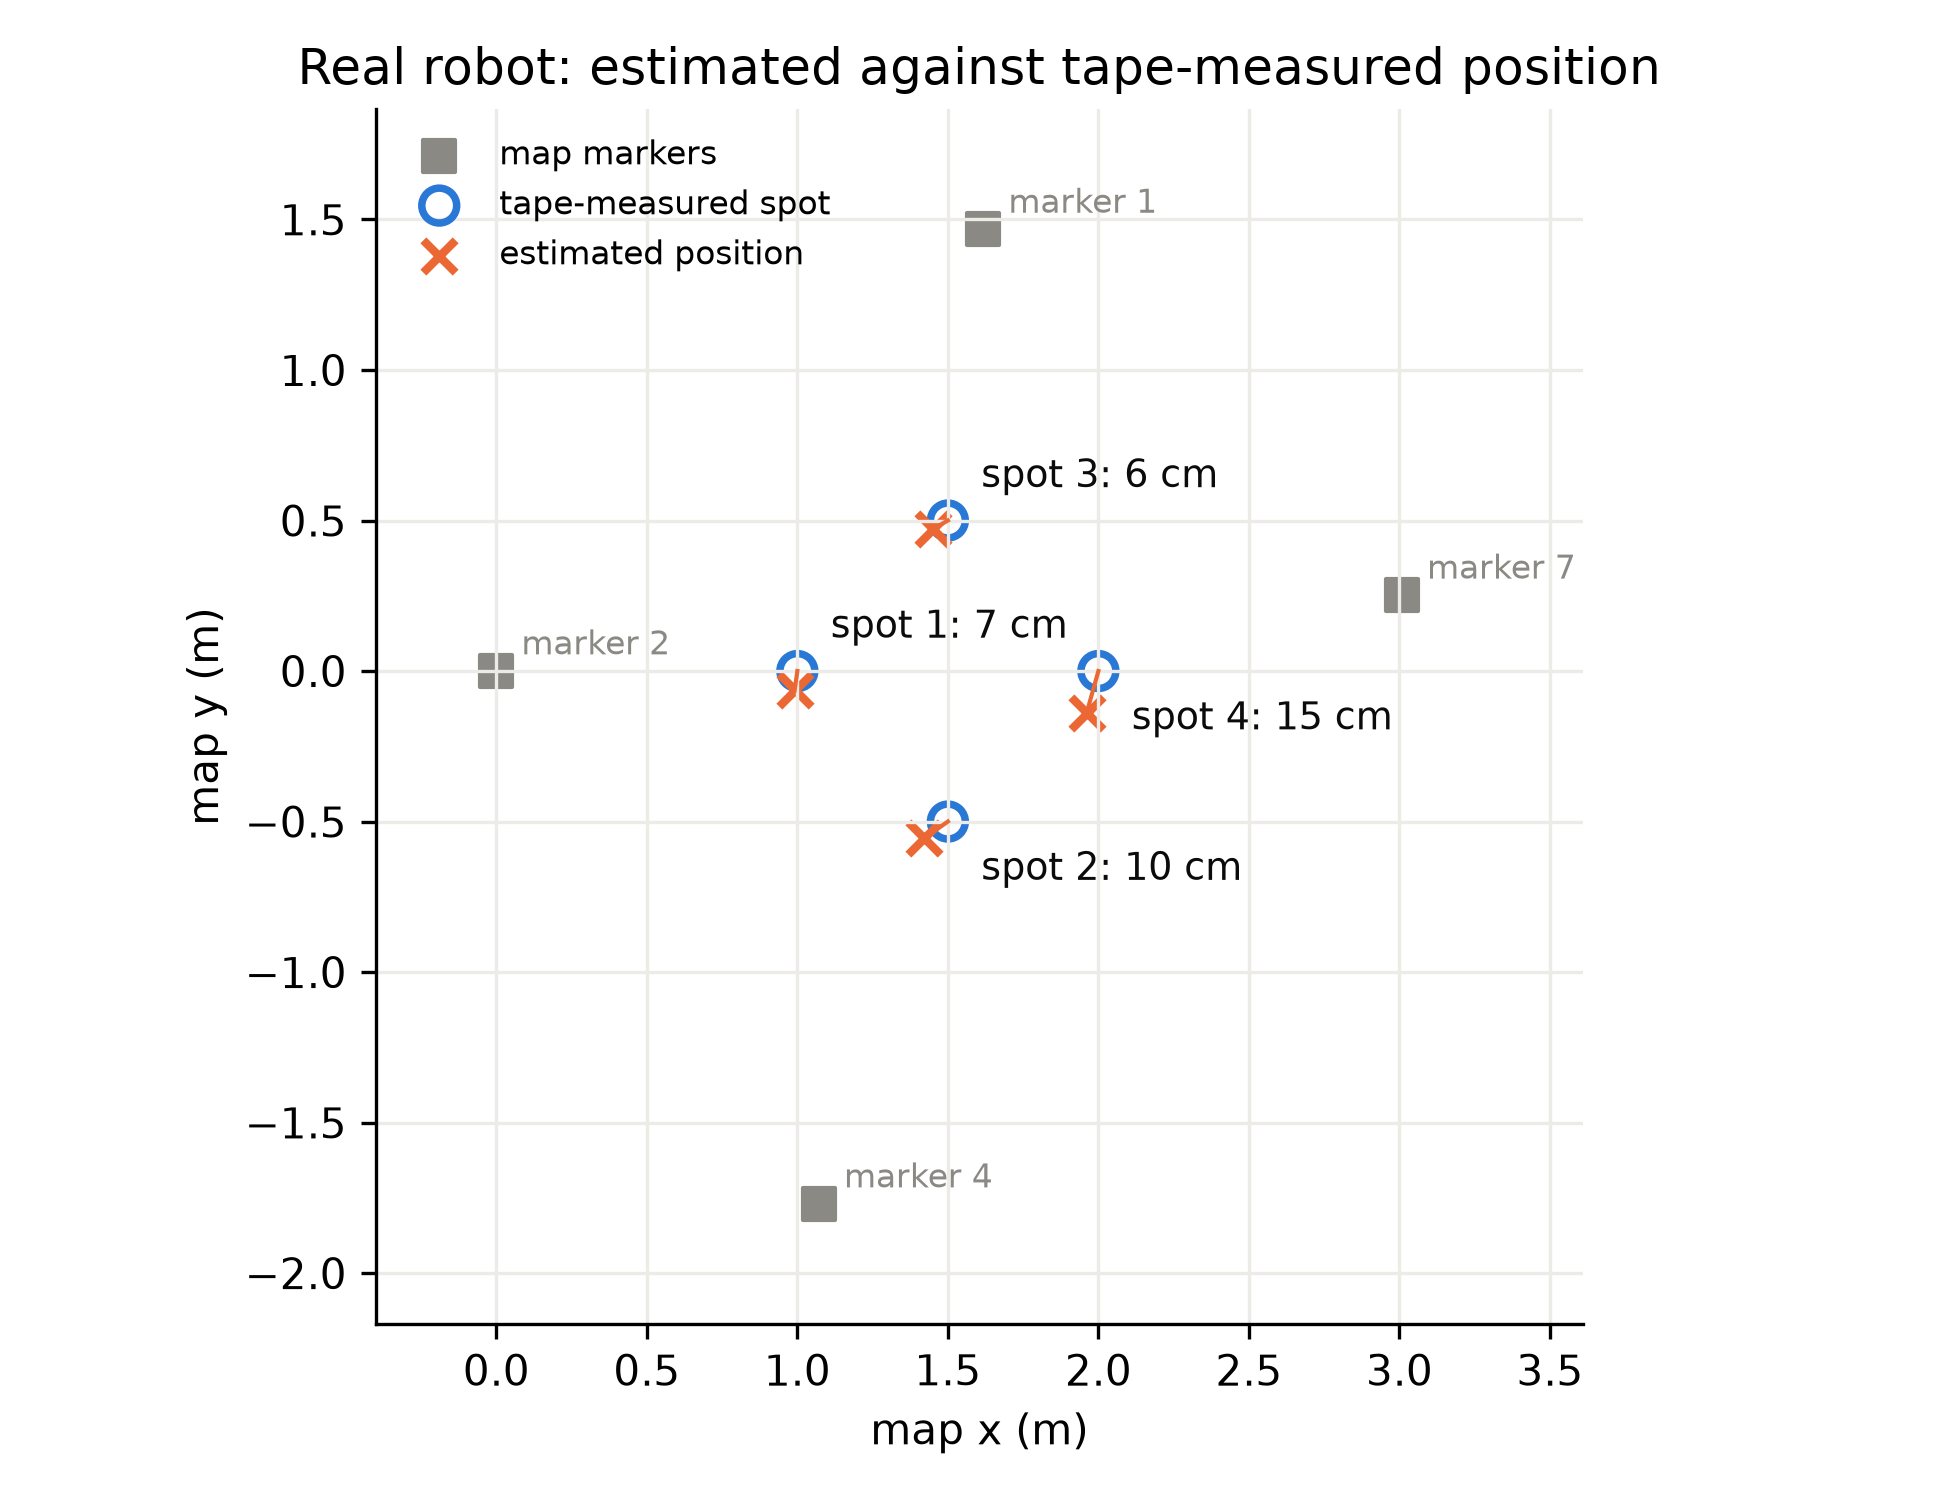
\includegraphics[width=\columnwidth]{figures/spot_accuracy.png}
\caption{Real robot: estimated positions (crosses) against tape-measured spots (circles), with the mapped markers.}
\label{fig:spots_result}
\end{figure}

\begin{table}[t]
\centering
\caption{Real robot at four tape-measured spots}
\label{tab:l3}
\setlength{\tabcolsep}{4pt}
\begin{tabular}{@{}llll@{}}
\toprule
Spot & Measured (m) & Estimated (m) & Error (cm) \\
\midrule
1 & $(1.00, 0.00)$ & $(0.991, -0.065)$ & 6.5 \\
2 & $(1.50, -0.50)$ & $(1.421, -0.555)$ & 9.6 \\
3 & $(1.50, 0.50)$ & $(1.450, 0.472)$ & 5.7 \\
4 & $(2.00, 0.00)$ & $(1.960, -0.141)$ & 14.6 \\
\midrule
Mean & & & 9.1 \\
\bottomrule
\end{tabular}
\end{table}

\subsection{Assumptions and problems}
The filter assumes a flat floor, a static map and markers that do not move, and it treats the measurements of different markers as independent. The real-robot errors are measured against tape measurements, which themselves carry an error of about a centimetre, and against a map built from phone videos.

The first attempt at the real-robot test gave errors of 1.5 to 7\,m. The driver reads the arm and the wheels in one call, and the arm servos repeatedly stopped answering on the shared servo bus, so whole control steps were skipped and no wheel velocities were published. The odometry froze while the robot drove, the filter received no motion, and it settled on poses that fit single markers seen from new places. The bus errors did not occur in a second run, which gave the results above. The failed run shows how much the filter depends on odometry between marker sightings. Other problems were practical: the camera's device number changed after the cables were replugged, the camera tilt had to be corrected as described above, and a stray marker with an id outside the map (37) appeared in one distance measurement.

% =====================================================================
\section{Conclusion}
\label{sec:conclusion}
The particle filter localized the LeKiwi to about 10\,cm in simulation and on the real robot. In simulation, it found the robot from a uniform start in 9.2\,s and kept a mean error of 8.9\,cm and 1.9\,$^\circ$, while odometry alone accumulated 5.8\,$^\circ$ of heading error in under two minutes. On the real robot, the estimates were within 5.7 to 14.6\,cm (mean 9.1\,cm) of four tape-measured spots. The camera calibration had a reprojection error of 0.41\,px, and within 1.5\,m the detected markers agreed with the map to about 1\,cm. The weak points are the range, where marker errors grow to 6\,cm at 2\,m and 7\,cm at 5\,m, a scale error of 3.7\,\% in the detected distances that the calibration likely introduced, and the filter's dependence on uninterrupted odometry, which the servo bus failure showed. Recalibrating with a rigid board, using the weighted mean or a clustering of the particles as the estimate, and decoupling the wheel readings from the arm in the driver would address these.

\begin{thebibliography}{14}

\bibitem{clark6b}
C.~Clark, ``Lecture 6B: Localization I,'' ROB-GY 6003 Foundations of Robotics, New York University, Brooklyn, NY, USA, 2026.

\bibitem{gordon1993}
N.~J. Gordon, D.~J. Salmond, and A.~F.~M. Smith, ``Novel approach to nonlinear/non-Gaussian Bayesian state estimation,'' \emph{IEE Proc. F (Radar and Signal Processing)}, vol.~140, no.~2, pp.~107--113, 1993.

\bibitem{dellaert1999}
F.~Dellaert, D.~Fox, W.~Burgard, and S.~Thrun, ``Monte Carlo localization for mobile robots,'' in \emph{Proc. IEEE Int. Conf. Robotics and Automation (ICRA)}, 1999, pp.~1322--1328.

\bibitem{thrun2005}
S.~Thrun, W.~Burgard, and D.~Fox, \emph{Probabilistic Robotics}. Cambridge, MA, USA: MIT Press, 2005.

\bibitem{clark7b}
C.~Clark, ``Lecture 7B: Particle filters,'' ROB-GY 6003 Foundations of Robotics, New York University, Brooklyn, NY, USA, 2026.

\bibitem{lerobot}
R.~Cadene, S.~Alibert, A.~Soare, Q.~Gallouedec, A.~Zouitine, and T.~Wolf, ``LeRobot: State-of-the-art machine learning for real-world robotics in PyTorch,'' 2024. [Online]. Available: \url{https://github.com/huggingface/lerobot}

\bibitem{garrido2014}
S.~Garrido-Jurado, R.~Mu\~{n}oz-Salinas, F.~J. Madrid-Cuevas, and M.~J. Mar\'{\i}n-Jim\'{e}nez, ``Automatic generation and detection of highly reliable fiducial markers under occlusion,'' \emph{Pattern Recognition}, vol.~47, no.~6, pp.~2280--2292, 2014.

\bibitem{macenski2022}
S.~Macenski, T.~Foote, B.~Gerkey, C.~Lalancette, and W.~Woodall, ``Robot Operating System 2: Design, architecture, and uses in the wild,'' \emph{Science Robotics}, vol.~7, no.~66, Art. no. eabm6074, 2022.

\bibitem{todorov2012}
E.~Todorov, T.~Erez, and Y.~Tassa, ``MuJoCo: A physics engine for model-based control,'' in \emph{Proc. IEEE/RSJ Int. Conf. Intelligent Robots and Systems (IROS)}, 2012, pp.~5026--5033.

\bibitem{for26}
R.~Khorram Bakht, ``FoR26: Course repository for ROB-GY 6003, Assignment 4: Localization with ArUco markers,'' 2026. [Online]. Available: \url{https://github.com/lair-research-nyu/FoR26/tree/assignment4}

\bibitem{zhang2000}
Z.~Zhang, ``A flexible new technique for camera calibration,'' \emph{IEEE Trans. Pattern Anal. Mach. Intell.}, vol.~22, no.~11, pp.~1330--1334, 2000.

\bibitem{bradski2000}
G.~Bradski, ``The OpenCV library,'' \emph{Dr. Dobb's Journal of Software Tools}, 2000.

\bibitem{collins2014}
T.~Collins and A.~Bartoli, ``Infinitesimal plane-based pose estimation,'' \emph{Int. J. Comput. Vision}, vol.~109, no.~3, pp.~252--286, 2014.

\bibitem{kitagawa1996}
G.~Kitagawa, ``Monte Carlo filter and smoother for non-Gaussian nonlinear state space models,'' \emph{J. Comput. Graphical Statist.}, vol.~5, no.~1, pp.~1--25, 1996.

\end{thebibliography}

\end{document}
